\section{Introduction}

%Offensive language and out-of-topic discussions give the impression that humans are unable to debate in the feeling of pseudonymity.

Online news outlets are drowning in the vast quantity of user comments. While there are certainly high-quality comments that, i.e., give a new perspective to a story, there are as well comments which are rather unwelcome. They range from out-of-topic discussions to use of offensive language. A large number of websites are closing their comment sections because they cannot cope with the sheer amount of user-generated content. News organizations already have economic difficulties\footnote{\url{https://en.wikipedia.org/wiki/Decline_of_newspapers}} and they cannot afford to moderate comments. However, with the help of new Natural-Language Processing (NLP) and machine learning techniques, there is hope to automatically analyze user comments. As a consequence, it frees up resources from moderation and opens the comment sections again. 

There already exist works to detect hate speech or abusive language in user-generated content \cite{hateoffensive, risch_delete_nodate, Nobata:2016:ALD:2872427.2883062, schmidt2017survey}. In this work, we want to take a different perspective on the issue. Instead of eliminating `bad' we want to identify high-quality (or `good') comments. We achieve this by classifying according to fine-grained criteria that constitute those comments. Such criteria are, for instance, whether a comment is about the topic of the article or if it supports its claims with an argument. In this master's thesis, we want to achieve a higher precision and recall on classifications on corpora of news comments reported in the scientific literature. The detailed description of what classes we want to predict on which datasets are given in further sections. The successful classification of specific fine-grained criteria allows us to (hopefully) detect high-quality comments. For the assignment of which criteria belongs to `bad' comments or `good', we rely on research in the field of media studies.

In contrast to prior work, we assume that the article and other comments are important to be considered when making classifications. To illustrate our motivation, we take two humanly-annotated comments from a Canadian newspaper \cite{kolhatkar2018sfu}: ``Time for the elders and chiefs to stand up to the plate and take a leadership role!". This comment is labeled as constructive (or in other words: high-quality) and ``Maybe this will motivate the cabbies in TO to clean their filthy cars! That are a disgrace.'' This is labeled as non-constructive. For us as humans, it is hard to make a judgment without reading the article first. Moreover, the annotators were required to read the article first before deciding whether an article is constructive or not. So we should be fair and also give the machine the possibility to obtain the context before classifying.

 \begin{figure}
 \vspace*{0.2in}
 \hspace*{-0.1in}
 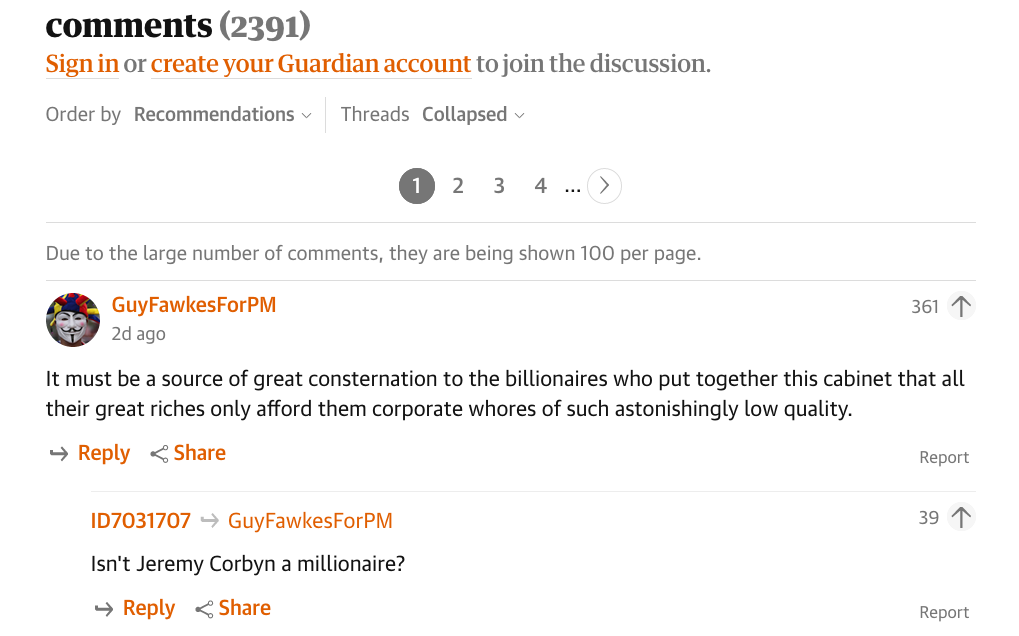
\includegraphics[width=0.5\textwidth]{comments}
      \caption[Caption for LOF]{An opinion article of the Guardian about the UK Prime Minister Theresa May received 2391 comments within two days.\protect\footnotemark}
    \label{fig:model}
\end{figure}

\footnotetext{\url{https://www.theguardian.com/commentisfree/2018/oct/03/the-guardian-view-on-theresa-mays-speech-getting-by-on-borrowed-time}}

In order to formally define the problem, let $C$ and $A$ be the set of all comments and articles respectively. In addition, we define: 
\\\\
$\text{isArticle}=\{(c, a)| \forall (c,a) \in C \times A: c\text{ is a comment of }a\}$
\\
$\text{isSurrounding}=\{(c, o, a)| \forall (c,o, a) \in C \times C \times A:$

$\quad\text{isArticle(}c, a\text{)} \wedge \text{isArticle(}o, a\text{)} \wedge  c \neq o\}$
\\\\
The training set $T =\{(c_n, a_n, s_n, y_n)\}^N_{n=1}$ consists of quadruple-wise data, where $c \in C$, $a \in A$, $s \subseteq \{o | \forall o \text{ isSurrounding(}c,o,a)\}$ and $(c, a) \in \text{isArticle}$. In addition, $y \in Y $ is the corresponding label for $Y=\{1,..., l\}$ classes. We wish to learn a classifier $\gamma$ that maps a comment, its article, and its surrounding comments to classes: $\gamma: C \times A \times C^* \rightarrow Y.$

% TODO: describe the formula so humans understand it

% \begin{figure}
%% \vspace*{0.2in}
%% \hspace*{-0.1in}
% 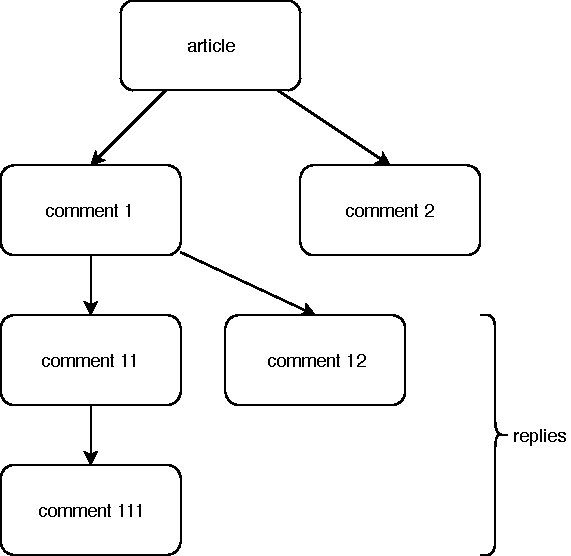
\includegraphics[width=0.5\textwidth]{tree}
%      \caption{df}
%    \label{fig:tree}
%\end{figure}

%large number of people does not necessarily lead to justified judgments – as seen for instance in the Brexit referendum.

In addition, we present a method of harnessing user votes to derive a comparable popularity score for each comment. We assume that the popularity of a comment is a rough proxy for its quality. So, with a comparable score, we can, i.e., divide comments into high-quality and low-quality comments. Nevertheless, we are aware that a high number of up-votes does not necessarily indicate a good comment. A German right-wing internet group `Reconquista Germanica'\footnote{\url{https://en.wikipedia.org/wiki/Social_media_disruption_by_far-right_groups_in_Germany}} coordinates attacks on their political opponents -- among other things -- in the comment section. They flood it with racist remarks and also up-votes them. Consequently, considering those comments and votes may lead to confounding good with racist. However, we still assume that, especially in an enormous corpus, the vote of the crowd has a meaning. News aggregators such as Hacker News\footnote{\url{https://news.ycombinator.com/}} or Reddit\footnote{\url{https://www.reddit.com/}}, live from their user votes to identify high-quality content. Still, there are a lot of factors that come into play when people vote and our method only operates on the number of votes at one specific moment in time. We neither know who casts these votes nor when. This may not be enough to come to a reasonable, objective, and comparable popularity score. We will critically investigate our method on multiple existing comment datasets before drawing conclusions.

So what is the bigger picture of user comments? Why exactly is it important to have them? Glenn Greenwald\footnote{\url{https://theintercept.com/2017/12/18/comments-coral-project/}} states:
\begin{quote}
``Journalists often tout their responsibility to hold the powerful accountable. Comments are a way to hold journalists themselves accountable.''
\end{quote}

So, one facet is about controlling the journalists themselves. Before the Internet, people could only send letters to the editors to express their opinions. A fraction of those letters was printed but those letters were obviously moderated strictly. Thus, the introduction of online news comments was an emancipatory act of depriving journalists of their role as gatekeepers. For the first time, a debate about an issue could happen in the wider public. This touches on the discourse ethics\footnote{\url{https://en.wikipedia.org/wiki/Discourse_ethics}} as proposed by J{\"u}rgen Habermas into practice. The principle of discourse ethics is that a group of people with a rationale debate comes to a common conclusion which manifests the morale. This is a stark contrast to Immanuel Kant's categorical imperative which focuses on individuals' convictions. The theoretical concept of the discourse ethics can be set in practice in the comment section albeit in some variation. In essence, it is about the belief that the collective can come to better conclusions than a sole person. The journalist who wrote the article has a limited view on the issue. Over the course of the debate in the comment section, all participants will eventually reach a common conclusion. But to do so, they have to follow specific discourse rules -- an idealistic scenario. Nevertheless, J{\"u}rgen Habermas, and other philosophers, thoughts can help us to answer fundamental questions.

The field of journalism is tightly coupled with the technological advancement of our society. Only through the invention of the letterpress by Johannes Gutenberg could humans spread information so fast. This allowed the journalistic profession to establish and flourish. The ongoing digital revolution also affects journalists and there is a long tradition of supporting their work with digital technologies. It started in the late 1960s with computer-assisted reporting\footnote{\url{https://en.wikipedia.org/wiki/Computer-assisted_reporting}} and lead to current ideas about automatic reporting\footnote{\url{https://en.wikipedia.org/wiki/Automated_journalism}}. Right now, there is a larger effort by supporting newspapers in managing their user comments. On example is the unprecedented Coral Project\footnote{\url{https://coralproject.net/}}, a cooperation among Mozilla, the New York Times and the Washington Post, that interviewed more than 400 experts in 150 newsrooms to develop an IT system to manage comments. In the following section, we give a detailed overview of related scientific work of machine-learning-based natural-language processing on news comments.

\section{Related Work}

The literature that is related to this work can be roughly split into two categories. One is about news comments and machine learning applied to it. And the second is about recent trends in NLP with deep learning.

\subsection{News Comments}
With the beginning of Web 2.0, there is an abundance of user-generated content. Some influential earlier work analyzed comments on Digg\footnote{\url{http://digg.com/}} \cite{Gomez:2008:SAS:1367497.1367585, Lampe:2004:SBD:985692.985761}, or predicted the popularity of online content on Youtube and Digg \cite{Szabo:2010:PPO:1787234.1787254} or Reddit \cite{Rizos:2016:PNP:2872518.2890096}. Coming from the area of human-computer interaction, Park et al. \cite{Park:2016:SCM:2858036.2858389} build a system to manage comments by incorporating traditional, feature-based machine learning.

Recent work focused on identifying moderator-picked comments on New York Times website, so-called \textit{NYT Picks}. Nicholas Diakopoulos \cite{diakopoulos2015picking} presents nine criteria for comments that distinguish NYT Picks from non-NYT Picks. Three criteria can be computed. Kolhatkar and Taboada \cite{kolhatkar_using_2017} predict the NYT Picks with traditional, feature-based machine learning as well as deep learning. They achieved an F1 score of $0.84$. In their follow-up work, they constructed the \textit{SFU Opinion and Comments Corpus} \cite{kolhatkar2018sfu}, where they labeled over 1000 comments for \textit{constructiveness} and they achieve an accuracy of $72.59\%$ \cite{kolhatkar2017constructive}. They define constructive as: 
\begin{quote}
     ``Constructive comments intend to create a civil dialogue through remarks that are relevant to the article and not intended to merely provoke an emotional response. They are typically targeted to specific points and supported by appropriate evidence.''
\end{quote}
Napoles et al. \cite{napoles2017automatically} focused on detecting `good' discussions on a comment thread level. They define `good' discussions as ERIC: Engaging, Respectful, and/or Informative Conversation. They as well created a corpus of comments, the \textit{Yahoo News annotated comments corpus} \cite{napoles2017finding}, labeled a subset of about 10k comments and  2.4k threads and predicted ERIC threads with an F1 score of $0.73$. For German,  Schabus et al. \cite{Schabus:2017:OMP:3077136.3080711} constructed a dataset of comments and annotated over 11k of them. They present several approaches and experiment with features-based as well as deep learning based. In their follow-up paper Schabus and Skowron \cite{schabus_academic-industrial_nodate} describe how they resort to a feature-based machine method for usage in a production system. A detailed comparison of all related datasets is presented later in Section~\ref{sec:commcorp}.

The work so far did not consider the context of an article. Namely, the article and also other comments. The very recent of work by Cheng et al. \cite{2018arXiv180807191C} considers the abstract of the news article as well as surrounding comments to classify comments. It adapts the text matching methods of Wang et al. \cite{wang_bilateral_2017} that uses an LSTM \cite{hochreiter1997long} with attention mechanism. However, their work has one weakness. They interpret all comments with over 10 up-votes as positive and the rest as negative samples in a binary classification problem. This is a gross simplification for multiple reasons. For instance, earlier comments are more likely to get more up-votes. So they may only predict comments that appear earlier in the discussions than others. Even though they achieved an accuracy of 70.75\% and an F1 score of 0.8073, their true contribution is unclear. Nevertheless, their deep learning network architecture of combining comment, article, and other comments can be a starting point for our work.

There has been significant work on detecting hate speech and offensive language with NLP. A closer look is out of the scope of this thesis and the interested reader is guided to a survey by Schmidt and Wiegand \cite{schmidt2017survey}. In particular, one paper by Gao and Huang \cite{Gao_2017} is worth mentioning because they work on context-aware classification. They as well point out that work on comments neglects its context. They developed an architecture of three parallel LSTMs, one for the text, one for the author, and one for the article. The three LSTMs are combined into a classifier. They constructed their own datasets of annotated tweets that relate to news articles. In their experiments, they claim that their context-aware model outperforms the one without context. Unfortunately, they did not apply their method to a commonly used dataset to put their contribution into perspective. 

Loosely related is the work by Qin et al. \cite{2018arXiv180503668Q} who automatically generate high-quality comments. Also, the problem of \textit{stance detection} is related. In this field, it is about detecting whether a response to a statement is affirmative or opposing. Some promising work has been carried out by Kochkina et al. \cite{kochkina2017turing}. In addition, the prediction of the helpfulness of user products reviews done by Singh et al. \cite{SINGH2017346} is relevant. Another work on product reviews and recommender system has been done by Zheng et al. \cite{Zheng:2017:JDM:3018661.3018665}. They encoded the product description as well as reviews with an LSTM respectively before combining the two sub-networks into a classifier. 

Outside of the computer science community, there exists qualitative analysis of comments that should guide our work. Loosen et al. \cite{loosen_making_2017} formulated several comment quality indicators after conducting interviews with news professionals as well as developing a software mockup. Among other things, they list `comment length' and `readability' but also the `reference to the article' and `references to other comments' as an indicator. Their work is built upon earlier research done by Diakopoulos et al. \cite{Diakopoulos:2011:TQD:1958824.1958844} and Noci et al. \cite{noci2012comments}. There is also an abundance of comment guidelines that outline good comments. The New York Time writes in their guidelines\footnote{\url{https://help.nytimes.com/hc/en-us/articles/115014792387-Comments}}: ``We are interested in articulate, well-informed remarks that are relevant to the article.'' Also, the community guidelines by the Guardian requires commentators to ``[k]eep it relevant''\footnote{\url{https://www.theguardian.com/community-standards}}.

So the relation to the article plays a role when judging comments for its quality. Current machine learning methods often are too simplistic and neglect this feature all-together.

\subsection{Transfer Learning with Language Models}

Transfer learning describes methods on how to re-use (intense) computations on downstream tasks. Pre-trained word embeddings, as popularized by Word2Vec \cite{DBLP:journals/corr/abs-1301-3781}, GloVe \cite{Pennington14glove:global} or fastText \cite{bojanowski2017enriching}, are one example of transfer learning in NLP. Within the deep learning NLP community, there is a trend of abandoning word embeddings in favor of text representations derived from pre-trained language models. There are two main reasons for this: first, the word tokens are global which means that they are context-agnostic. This is a drawback because there might be multiple meanings for a word. For instance, `bank' can describe a financial institution or an embankment. The true meaning in a sentence can only be inferred by considering the context. Second, the meaning of the word is lost after the embedding layers. Subsequent, deeper layers do not have access to the `meaning' of a word that was injected through the word embeddings.

Language Models (LM) try to predict the next word based on previous words. This is a challenging task. In such a manner, the model has to learn the nuances of a language over long sequences of text. A good thing is that they do not require annotated data and there is an abundance of raw text freely available (e.g. from Wikipedia). After training an LM, there is the hope of transforming its capabilities to other tasks. The Elmo embeddings by Peters et al. \cite{peters2018deep} use the potential of LM to surpass earlier work on contextual word embeddings by McCann et al. \cite{mccann2017learned} (CoVe). They use the internal state of a language model to obtain vectors as a building block that can directly replace traditional word embeddings. Similar work has been done by of Abkib et al. \cite{akbik_contextual_nodate} for Flair\footnote{\url{https://github.com/zalandoresearch/flair}}. Peters et al. \cite{peters_dissecting_2018} describe LMs and their use in text representation in more detail in their recent publication.

Howard and Ruder show with Ulmfit \cite{howard_universal_2018} how to apply transfer learning to fine-tune from an ordinary LM to downstream classification task. They achieved multiple state-of-the-art performances on text classification\footnote{\url{http://nlpprogress.com/text_classification.html}} and sentiment detection\footnote{\url{http://nlpprogress.com/sentiment_analysis.html}}, e.g. on the IMDb dataset\footnote{\url{https://ai.stanford.edu/~ang/papers/acl11-WordVectorsSentimentAnalysis.pdf}}. In contrast to Elmo, Ulmfit consists of a full architecture and methodology to apply text classification to real-world data. They point out that the challenging part is the method of how to fine-tune from the LM to the task. The OpenAI transformer by Radford et al. \cite{radford2018improving} also starts with a trained LM and \textit{transforms} it to downstream tasks. Their performance for text classification is below than Ulmfit. But they provided also ways to transform the LM to other tasks such as question answering. Both papers highlight that there is far more to explore in the field of LM fine-tuning. There is a comparison of several approaches done by Perone et al. \cite{2018arXiv180606259P} -- unfortunately without Ulmfit or the OpenAI transformer.

Transfer learning in NLP is currently a hot topic and there might be no clear answers yet. There are also other approaches without LM, i.e., the `Universal Sentence Encoder' by Cer et al. \cite{cer2018universal}. They also create context-aware text representation but build upon their prior work about a custom artificial neural network architecture.


\section{Context-aware Classification of News Comments}
\label{sec:methods}

%In order to select comments that are worth promoting, we use a two-step process. First, we select `good' comments. Then we further filter those comments and promote only a selection to avoid duplicates.

%\subsection{Identifying `Good' Comments}


%\subsection{Clustering `Good' Comments}
%
%For the second part, we cluster those comment and present only one (most likely the first one) out of each cluster. We will use topic modeling to find the clusters [not sure which one]. Right now it is open how to rank the comments. We may need additional labeled data for it or just refrain to a time-based ordering for the good comments.


We want to draw from ideas of the recent developments in NLP to classify news comments considering their context. We propose and evaluate several deep learning architectures. We interpret the problem as a combination of text classification and text matching. We follow the recent advancements of language model fine-tuning as done by Ulmfit \cite{howard_universal_2018} and the OpenAI Transformer \cite{radford2018improving}. We will first present several context-unaware baselines approaches before describing our context-aware architectures.

\subsection{Baseline Models}

The baseline methods range from traditional feature-based approaches to well-established deep learning approaches.
All of them do not have the context of the article. For the features, the work by Kolhatkar and Taboada \cite{kolhatkar_using_2017} with features such as average word/sentence/comment length is a starting point. And also stylometric features as described by Potthast et al. \cite{2017arXiv170205638P} should help to distinguish certain quality criteria. Most importantly we use well-established, i.e., attention-based deep learning architectures. Further, we will use text classification with the original Ulmfit \cite{howard_universal_2018} solely on the comment's text. This way we have to ensure that the additional context is useful.
\subsection{Context-aware Models}

We propose three different directions for context-aware models. For the beginning, we limit the models to only consider the article as context and not the surrounding comments.
First, we start with simple architectures using multiple recurrent neural networks, i.e., LSTMs, in parallel. One for the comment and one for the article before joining together in a fully connected layer. This follows the work of Gao and Huang \cite{Gao_2017} who used it to classify hate speech tweets. Or Zheng et al. \cite{Zheng:2017:JDM:3018661.3018665} who used it for product reviews.

 \begin{figure}
 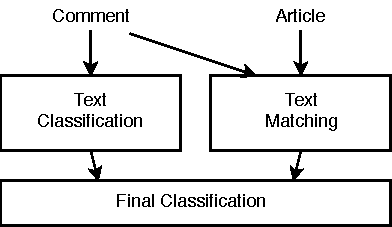
\includegraphics[width=0.5\textwidth]{ma}
   \caption{Overview of the model architecture.}
    \label{fig:model}
\end{figure}

Second, we propose a model architecture consisting of two sub-networks, one only on the comment's text and one also for the text matching between the article's text and the comment's text. Both sub-structures are combined into a final layer to classify the comments. For the text classification, we follow the work of Ulmfit \cite{howard_universal_2018}. For the text matching, we follow the work of the OpenAI transformer \cite{radford2018improving}.  Text matching describes the general research problem whether two texts match while the matching criteria can be defined. Examples of text matching are question answering. So the general idea is that we first train a general language model on a large text corpus. Then, transform and fine-tune the trained language model to our task. An overview of the complete architecture is shown in Figure~\ref{fig:model}. The whole process of fine-tuning looks as follows:

\begin{enumerate}
   \item Train a language model on a large, un-labeled corpus (or use a pre-trained one)
   \item Re-train the language model on an un-labeled corpus of comments
   \item Fine-tune the model on a labeled sub-set of comments
 \end{enumerate}
 
Third, we want to experiment with whether classification criteria `off-topic' can be solved as a text matching problem. To our knowledge, this has not tried out so far. This would make the complex two-step architecture proposed in the previous paragraph superfluous.

\newpage

\subsection{Further Ideas}

To further improve the model, we could incorporate external knowledge into our model. Some concrete information about people and e.g. their affiliation, i.e., political party membership, may not be in the training data. One way would be to use a Named-Entity Recognition (NER) method and then to look up the entity on external knowledge resources such as Wikipedia or Wikidata.


\section{Data}

%\tablefootnote{\url{https://github.com/sfu-discourse-lab/SOCC}},
%\tablefootnote{\url{https://github.com/cnap/ynacc}}\cite{napoles2017finding}
%\tablefootnote{\url{https://ofai.github.io/million-post-corpus/}}

In this section, we will give an overview of available partly-annotated data sources as well as a method to harness user votes.

\subsection{Corpora of News Comments}
\label{sec:commcorp}
\begin{center}
\begin{table}
  \begin{tabular}{| p{2cm} | p{2.8cm} | p{2.7cm} |}
    \hline
    Dataset & Description & Annotations \\ \hline
    SFU Opinion and Comments Corpus \cite{kolhatkar2018sfu} (SOCC), in English & 10k articles with their 663k comments from 303k comment threads, from 2012 to 2016, from Canadian newspapers, with up- and down-votes & 1,043 comments in responses to 10 articles, labeled for constructiveness and toxicity \\ \hline
    Yahoo News Annotated Comments Corpus \cite{napoles2017finding} (YNACC), in English & 522k comments from 140k threads posted in response to Yahoo News articles, with up- and down-votes & 9.2k comments labeled for agreement, audience, persuasiveness, sentiment, tone, (off-)topic and 2.4k threads labeled for agreement, constructiveness, type \\ \hline
        One Million Posts Corpus \cite{Schabus:2017:OMP:3077136.3080711, schabus_academic-industrial_nodate} (OMPC), in German & 12k articles, 1M comments, from an Austrian Newspaper, with up- and down-votes & 11k comments with the following labels: sentiment, off-topic, inappropriate, discriminating, feedback, personal studies, argument used \\ \hline
        Tencent News Corpus (TNC) by Qin et al. \cite{2018arXiv180503668Q}, in Chinese &  200K articles and 4.5M comments, from a Chinese news website, 2017, with up-votes & 40k comments labeled for quality (from 1 to 5) \\ \hline
  \end{tabular}
  \caption{Overviews about annotated corpora of comments.}
  \label{table:datasets}
  \end{table}
\end{center}
There exists four corpora of news comments where part of the comments are annotated for its quality. Table~\ref{table:datasets} gives an overview about them, two are in English, one in German and in Chinese.

For our work, the YNACC and the OMPC are especially interesting because of their fine-grained annotations. The number of annotated comments in SOCC are too few. TNC has enough data but only one label of quality. YNACC and OMPC have also some overlapping annotation criteria: off-topic and sentiment. This allows us to compare the same method with identical labels on both datasets. Since YNACC contains English and OMPC German comments, we can test our approach on two languages.

Besides, all of the corpora contain comment-level user votes. In order to make use of them, a method is presented in the next section.

\subsection{Harnessing User Votes}
\label{sec:data_votes}

News comments allow people to express their opinion about news articles. In the same breath, users are also able to vote on other users' comments. This can be interpreted as a label of the popularity of a comment. However, a problem is that one cannot take the raw number of votes to compare comments. Articles that attract more readers than others receive more comments and also more votes. Comments posted shortly after the article publication are more likely to be read and consequently receive more votes. So to make use of user votes, they first need to be preprocessed to obtain a comparable popularity score. 

In our previous, unpublished work, we developed a method to create binary popularity labels out of up-votes as follows:

\begin{enumerate}
\item Remove non-root comments
\item Remove articles with few comments 
\item Remove articles with few up-votes
\item Sort comments chronologically
\item Only consider first $N$ comments per article
\item Calculate relative portion of up-votes for each comment under \textit{one} article
\item For each comment rank, classify the first $X$ comments as positive and the last $X$ comments as negative, whereby $X * 2 <= $ number of articles
\end{enumerate}

So we normalize the up-votes first and then, leave out the comments with an average score because we assume that there the `crowd' did not come to clear decision. Only the very popular and the very unpopular comments were used as positive and negative samples respectively. The constants $N$ and $X$ were derived empirically. In this master's thesis, we want to generalize this method and also determine $X$ and $N$ more scientifically. First, we split the whole process into two parts. The development of an objective popularity score and the method of turning this score into classes. Moreover, we want to adapt it to also work for down-votes. This enables us to use this approach on the datasets in Table~\ref{table:datasets} which have down-votes. For this two additional classes are required but how exactly the comments are assigned to a class is due to further research. 

Finding a way of harnessing user votes to get meaningful labels would allow us to have a magnitude more of annotated comments. Halevy et al. \cite{halevy2009unreasonable} showed that more data, in general, helps to improve the performance of deep learning models. So with this method applied to datasets as presented in Table~\ref{table:datasets} would give us more data. This gives us the possibility to train a model to detect `good' comments. A hope is that if you feed those data into a deep learning model, it picks of the general tendency and leaves out the outliers. However, these assumptions need to get evaluated and we will describe in the next section.

\section{Evaluation}

 We have two different sub-sections for the evaluation because our contribution is two-fold.

\subsection{Context-Aware Classification}
To test the performance of our proposed architectures as described in Section~\ref{sec:methods}, we compare it to our baselines results and results reported in the scientific literature. The authors of OMPC report baseline values \cite{schabus_academic-industrial_nodate} for all their classification criteria. The criteria `off-topic` with a prediction of 0.2579,  recall of 0.6241 and an F1 score of 0.3516 leaves room for improvement. Because our model has the relation between comment and article, it ought to achieve better results. Also, the majority of the other criteria have F1 scores ranging from 0.5 to 0.7 that show these problems are far from being solved. (There will be a paper from Hamburg available shortly, where they also work on the OMPC and report F1 scores). It is our goal to outperform all classifications on OMPC in respect to precision and recall (and thus F1 scores). The classification criteria are: sentiment, off-topic, inappropriate, discriminating, feedback, personal studies, argument used.

Unfortunately, there are no reported values for the comments in YNACC –-- only per thread level. For SOCC, the authors \cite{kolhatkar2017constructive} report an accuracy of 0.7259 for identifying `constructive' comments. We claim that the context of a comment is important for its classification. Since in the author's definition of constructive is implied, that it is relevant to the article, we have to outperform them to prove our approach works.

\subsection{Harnessing User Votes}
First, to evaluate our method as proposed in Section~\ref{sec:data_votes}, we compare the resulting classification against the annotated comments in Table~\ref{table:datasets}. There are certain labels such as `constructiveness', `argument used', or `on-topic' that should occur significantly more often in our `popular' comments. 

Second, we preprocess a dataset from Table~\ref{table:datasets} with our method and train a model, i.e., with a context-aware architecture. Then, we classify unseen comments. The final classification results are then evaluated by human annotators (10 articles, 100 comments, 5 people). With this, we can evaluate the whole multi-step process. We hope, that the combination of our harnessing method and the deep learning model can predict quality labels of comments.

Third, depending on the course of the master's thesis, we can conduct a larger user study. The study is with ten participants with a quantitative and a qualitative part to determine whether the `popular' comments are actually superior to other comments. First, participants are required to assign quality labels to comments after they read the corresponding article. Participants are asked to read three articles and judge ten comments per article. Second, in a semi-structured interview, we will try to elicit additional information about their decisions to get an understanding of what a good comment is in particular and how it relates to user voting on comments. 